\documentclass[11pt]{article}

% ---- Packages (all standard; compiles with pdflatex on TeX Live / MiKTeX / Overleaf) ----
\usepackage[utf8]{inputenc}
\usepackage[T1]{fontenc}
\usepackage[margin=1in]{geometry}
\usepackage{amsmath,amssymb,amsthm}
\usepackage{booktabs}
\usepackage{array}
\usepackage{enumitem}
\usepackage{xcolor}
\usepackage{mathtools}
\usepackage{graphicx}
\usepackage[hidelinks]{hyperref}

\definecolor{navy}{HTML}{0C1E3E}
\definecolor{gold}{HTML}{8B6914}
\definecolor{rust}{HTML}{8B3A0E}
\definecolor{sage}{HTML}{3F5A3B}

\newcommand{\vecx}{\operatorname{vec}}
\newcommand{\Cov}{\operatorname{Cov}}
\newcommand{\CVaR}{\mathrm{CVaR}}
\newcommand{\R}{\mathbb{R}}
\newcommand{\E}{\mathbb{E}}
\newcommand{\chiU}{\chi_{\mathrm{U}}}
\newcommand{\chiL}{\chi_{\mathrm{L}}}
\newcommand{\gco}{\mathrm{gCO_2eq/kWh}}

\title{\vspace{-2.2em}\textbf{\color{navy} Spatially-Correlated Distributionally Robust\\[2pt]
Scheduling for Carbon-Aware Data Centers}\\[6pt]
\large\color{gold} Phase 1 Results --- The Spatial Question, Resolved}
\author{Marco Ortiz Togashi \\ \small Supervisor: Prof.\ Bissan Ghaddar \\
\small IE School of Science \& Technology --- Capstone in Operations Research}
\date{June 2026}

\begin{document}
\maketitle
\thispagestyle{empty}

\begin{abstract}
\noindent This chapter closes the central Phase~1 question: does modelling the
\emph{spatial correlation} of carbon intensity across electrically coupled regions
improve a distributionally robust (DRO) data-center schedule? Extending the
methodology of the status report to \textbf{three} US/Canada cases that span the full
correlation spectrum, we find a \textbf{replicated, robustness-checked null}: the
joint spatial covariance never beats an independent (shuffled-marginals) baseline by
a material margin. The result is neither an artifact of weak correlation --- we first
\emph{validate} strong, de-seasonalized correlation in two interconnections --- nor an
assertion: a \textbf{mean-ablation experiment} shows the covariance signal is genuine
and exploitable but \emph{dominated} by the mean carbon field, and a
\textbf{tail-dependence} diagnostic shows the residual structure is non-elliptical
(upper-tail-independent, radially asymmetric) and therefore invisible to a
covariance-based ambiguity set by construction. Phase~1 thus delivers a
\emph{specification result} that directly motivates the Phase~2 copula extension.
\end{abstract}

\vspace{-0.5em}
\section{Headline}\label{sec:headline}

\begin{quote}\itshape\color{navy}
Spatial correlation of carbon intensity does not translate into robust scheduling
value: across the full correlation spectrum, in a Mahalanobis--Wasserstein DRO,
modelling the joint spatial distribution buys essentially nothing over treating each
region's carbon independently.
\end{quote}

\noindent Three findings make this a substantive, defensible result rather than a
bare negative:
\begin{enumerate}[leftmargin=1.4em,itemsep=2pt]
  \item \textbf{It is not absence of correlation.} We validate strong, residual-surviving
  correlation in two interconnections (\S\ref{sec:cases}); the DRO's spatial assumption
  \emph{is valid}. Validity of the assumption $\neq$ value from it.
  \item \textbf{It is not an edge case.} The null holds in the strongly-correlated cases,
  in an adversarial \emph{heterogeneous} case engineered to be diversifiable, and through
  a full robustness battery with multiple-testing correction (\S\ref{sec:gap}--\S\ref{sec:robust}).
  \item \textbf{We prove \emph{why}, causally.} A mean-ablation experiment
  (\S\ref{sec:ablation}) demonstrates the covariance is real but mean-dominated; a
  tail-dependence diagnostic (\S\ref{sec:tails}) shows the exploitable structure is
  non-elliptical.
\end{enumerate}

\section{The three cases: a correlation spectrum}\label{sec:cases}

We transport the \emph{identical} machinery of the status report --- Algorithm~2b
Mahalanobis--Wasserstein second-order cone program (SOCP), three nested constraint
regimes, $\CVaR_{0.95}$ metric, blocked 5-fold cross-validation to select the
Wasserstein radius $\varepsilon$, and a 1000-resample bootstrap confidence interval
on the spatial gap --- to three new region sets chosen to span the dependence
spectrum (Table~\ref{tab:cases}). All panels are hourly Electricity Maps lifecycle
carbon intensity, 2021--2025 ($43{,}824$ hourly observations per zone).

\begin{table}[h]\centering\small
\begin{tabular}{@{}llll@{}}
\toprule
\textbf{Case} & \textbf{Zones} & \textbf{Residual correlation} & \textbf{Mechanism} \\
\midrule
\texttt{us\_west} & CISO, BANC, LDWP, NEVP, AZPS & strong (0.72--0.78) & WECC: solar + weather \\
\texttt{taskc} & CA-ON, NYIS, MISO, PJM & strong (0.70--0.73) & East: weather fronts \\
\texttt{us\_hetero} & CISO, ERCO, BPAT & near-zero (ERCO--BPAT $0.00$) & solar / wind / hydro \\
\bottomrule
\end{tabular}
\caption{The three Phase~1 cases. \texttt{us\_hetero} is adversarial by design:
regions with different generation physics, chosen so their clean/dirty periods do
\emph{not} coincide --- if spatial DRO value exists anywhere, it should appear here.}
\label{tab:cases}
\end{table}

\paragraph{Correlation is genuine and survives de-seasonalization.}
Removing the per-zone hour-of-day mean (which collapses the spurious diurnal
co-movement seen in the California and Iberia sub-grids of the status report), the
two interconnected cases retain strong correlation: \texttt{us\_west}
CISO--NEVP $0.78$, CISO--LDWP $0.72$; \texttt{taskc} CA-ON--NYIS $0.73$,
MISO--PJM $0.70$. This confirms the hypothesis that interconnected US/Canada grids
carry real spatial carbon structure, unlike the European cases.
Figure~\ref{fig:summary} (and \texttt{figures/ci\_corr\_heatmap\_*}) shows the full
correlation matrices.

\section{The spatial gap: no robust value}\label{sec:gap}

The falsification test pairs the scheduler with either the \emph{joint} sample
covariance $\hat\Sigma$ or its \emph{block-diagonal} (cross-region-zeroed)
counterpart $\hat\Sigma^{\mathrm{shuf}}$; the out-of-sample $\CVaR_{0.95}$ gap
$\mathrm{shuf}-\mathrm{joint}$ measures the value of the spatial blocks (positive
$=$ joint better). The variable-capacity ceiling in regime~R2 uses bounds
$(x_{\min},x_{\max})=(50,75)$\,MW, calibrated to a loosely-binding regime on
\emph{training} data only (bind fraction $\approx 0.28$--$0.37$). Results in
Table~\ref{tab:gap}.

\begin{table}[h]\centering\small
\begin{tabular}{@{}lcccl@{}}
\toprule
\textbf{Case} & $\varepsilon^\star$ (CV) & \textbf{gap range (\% of $\CVaR$)} & \textbf{detectable} & \textbf{verdict} \\
\midrule
\texttt{us\_west}   & $1$ (8/9) & $-0.005$ \dots $+0.043$ & 1/9 (trivial, $+3\!\times\!10^{-6}\%$) & null \\
\texttt{taskc}      & $1$ (9/9) & $-0.022$ \dots $+0.038$ & 4/9, \emph{signs flip} across $\alpha$ & null (artifacts) \\
\texttt{us\_hetero} & $1$ (9/9) & $-0.233$ \dots $+0.062$ & 5/9, material ones \emph{negative} & null (joint \emph{hurts}) \\
\bottomrule
\end{tabular}
\caption{Spatial gap $\mathrm{shuf}-\mathrm{joint}$ in $\CVaR_{0.95}$, 9 cells per case
($3$ regimes $\times\ 3$ risk levels $\alpha$). Every gap is a small fraction of one
percent. CV selects $\varepsilon^\star=1$ throughout, so the DRO is genuinely engaged
--- this is not a ``model switched itself off'' null. In \texttt{us\_hetero} the only
detectable cells are \emph{negative}: estimating cross-region covariance that carries
no exploitable signal merely adds estimation noise.}
\label{tab:gap}
\end{table}

\section{Reliability: robustness battery, multiple testing, temporal stability}\label{sec:robust}

Each case was re-run with seasonal-residual, AR(1)-residual, and Ledoit--Wolf-shrinkage
covariance estimators. The largest $|\text{gap}|$ under \emph{any} estimator is
$0.07\%$ (\texttt{us\_west}), $0.18\%$ (\texttt{taskc}), $0.36\%$ (\texttt{us\_hetero})
of $\CVaR$ --- all economically negligible. No cell shows a \emph{material} beneficial
effect that is sign-stable across the seasonal \emph{and} AR(1) estimators; the cells
that flip positive disagree by orders of magnitude across estimators (e.g.\ \texttt{taskc}
R3/$\alpha 0.30$: seasonal $-0.033\%$ vs.\ AR(1) $+0.179\%$), the signature of
$\varepsilon$-selection noise.

\paragraph{Multiple testing.} Testing $144$ non-ablation cells, some bootstrap CIs
exclude zero by chance. Applying a Benjamini--Hochberg correction at $q=0.05$ over all
cells (bootstrap $p$-values), the largest \emph{positive} gap that survives is
$0.179\%$ --- precisely the AR(1) cell already rejected by the agreement rule. Nothing
material survives both criteria.

\paragraph{Temporal stability.} A walk-forward refit (train 2021--2023, test 2024)
reproduces the null: max $|\text{gap}|$ of $0.028\%$, $0.036\%$, $0.217\%$ across the
three cases. The result is not a 2025 artifact.

\section{Mean-ablation: the causal mechanism}\label{sec:ablation}

The preceding sections establish \emph{that} the covariance adds no value; this
experiment establishes \emph{why}. We neutralize the mean field $\bar\rho$ used for
\emph{scheduling} while keeping \emph{evaluation} on the real carbon panel. Two levels:
\textsc{level} equalizes each region's time-average to the global mean (keeping the
hour-of-day shape); \textsc{flat} sets a constant mean everywhere, so $\langle
\bar\rho, x\rangle$ is constant under fixed demand and the schedule is driven
\emph{purely} by the $\varepsilon\lVert L^{\!\top} x\rVert_2$ covariance penalty --- a
\emph{covariance-only world}. Results in Table~\ref{tab:ablation}.

\begin{table}[h]\centering\small
\begin{tabular}{@{}llll@{}}
\toprule
\textbf{Case} & \textbf{baseline} & \textsc{level} & \textsc{flat} (covariance-only) \\
\midrule
\texttt{us\_west}   & $\sim 0$, none det.\ & $\sim 0$, none & $\varepsilon^\star\!\to 0$;\ $-0.04$ \dots $+0.004$ \\
\texttt{taskc}      & $\sim 0$, sign-flips & $\sim 0$ & $\mathbf{+0.14}$ \dots $\mathbf{+0.41}$, \textbf{all 9 det.} \\
\texttt{us\_hetero} & negative & negative & $\mathbf{+0.39}$ \dots $\mathbf{+1.46}$, \textbf{all 9 det.} \\
\bottomrule
\end{tabular}
\caption{Mean-ablation. Equalizing the \emph{level} changes nothing --- the diurnal
mean shape still dominates. In the \emph{covariance-only} world the joint covariance
produces a material, fully-detectable advantage over the shuffled one, and CV no longer
collapses to a single $\varepsilon^\star$. The spatial covariance therefore \emph{does}
carry genuine, exploitable information --- it is simply \emph{swamped} by the mean in
the real problem. Identical gaps on a $2\times$ denser $\varepsilon$ grid confirm these
are not grid artifacts.}
\label{tab:ablation}
\end{table}

\noindent This converts the null from an assertion into a demonstrated \emph{ordering}:
\emph{the mean field dominates the schedule so completely that a real and exploitable
second-moment signal contributes negligibly.} The cost confirms it is not free lunch:
the \textsc{flat} schedule, by discarding the real mean, \emph{worsens} absolute
$\CVaR$ by $+1.9$--$4.1\%$ (\texttt{us\_west}) and $+1.6$--$3.8\%$ (\texttt{us\_hetero})
--- the covariance-only gain ($\le 1.46\%$) never repays it. \texttt{us\_west} is the
instructive exception ($\varepsilon^\star\!\to 0$, gap $\sim 0$): its strong
\emph{common-mode} positive correlation offers little even in isolation, because
diversification needs heterogeneity, not co-movement.

\section{Tail dependence: the structure the covariance cannot see}\label{sec:tails}

Why is even the exploitable-in-isolation covariance the \emph{wrong} object? Because
the genuine dependence lives in the tails and is non-elliptical. We estimate the
empirical upper/lower tail-dependence coefficients $\chiU$ (both regions \emph{dirty}
together --- the $\CVaR$-relevant co-movement) and $\chiL$ (both \emph{clean} together),
and compare $\chiU$ against the Gaussian-copula value at the matched correlation. A
Gaussian copula --- anything a covariance ball can represent --- has \emph{zero}
asymptotic tail dependence, so an empirical excess above it would be structure the DRO
misses.

\begin{table}[h]\centering\small
\begin{tabular}{@{}llccccc@{}}
\toprule
\textbf{Case} & \textbf{Pair} & $\rho$ & $\chiU^{\mathrm{emp}}$ & $\chiU^{\mathrm{Gauss}}$ & \textbf{excess} & $\chiL^{\mathrm{emp}}$ \\
\midrule
\texttt{us\_west}   & CISO\,$|$\,LDWP & $0.72$ & $0.25$ & $0.41$ & $-0.16$ & $0.48$ \\
\texttt{us\_west}   & BANC\,$|$\,LDWP & $0.65$ & $0.17$ & $0.35$ & $-0.18$ & $0.40$ \\
\texttt{taskc}      & CA-ON\,$|$\,NYIS & $0.73$ & $0.38$ & $0.42$ & $-0.04$ & $0.31$ \\
\texttt{us\_hetero} & ERCO\,$|$\,BPAT  & $0.00$ & $0.04$ & $0.05$ & $-0.02$ & $0.02$ \\
\bottomrule
\end{tabular}
\caption{Residual tail dependence at $q=0.95$. Two findings: (i) the empirical
$\chiU$ sits \emph{at or below} the Gaussian benchmark (excess $\le 0$) --- in the
dirtiest hours regions \emph{de-couple} (upper-tail independence), so there is nothing
in the dirty tail for a richer model to exploit; (ii) $\chiL > \chiU$ --- regions go
\emph{clean} together more than \emph{dirty} together. A Gaussian/elliptical copula
forces $\chiL=\chiU$, so this radial asymmetry is non-elliptical structure a
Mahalanobis--Wasserstein ball cannot encode.}
\label{tab:tails}
\end{table}

\section{Synthesis: why this is the expected outcome}\label{sec:why}

\begin{enumerate}[leftmargin=1.4em,itemsep=2pt]
  \item \textbf{The mean field dominates} (proven in \S\ref{sec:ablation}). The schedule
  is set by $\bar\rho$, shared identically by the joint and shuffled models; the
  covariance enters only as a second-order penalty.
  \item \textbf{Positive correlation is common, non-diversifiable risk.} Diversification
  value needs regions that hedge each other; real grids co-move, and the genuinely clean
  escape (Ontario; hydro BPAT) is already identified by its low \emph{mean}.
  \item \textbf{Even zero correlation does not help} (\texttt{us\_hetero}): with no
  cross-structure, fitting the joint covariance only adds estimation noise.
  \item \textbf{The exploitable structure is non-elliptical} (\S\ref{sec:tails}) ---
  invisible to a covariance/Wasserstein ambiguity set by construction.
\end{enumerate}

\begin{figure}[h]\centering
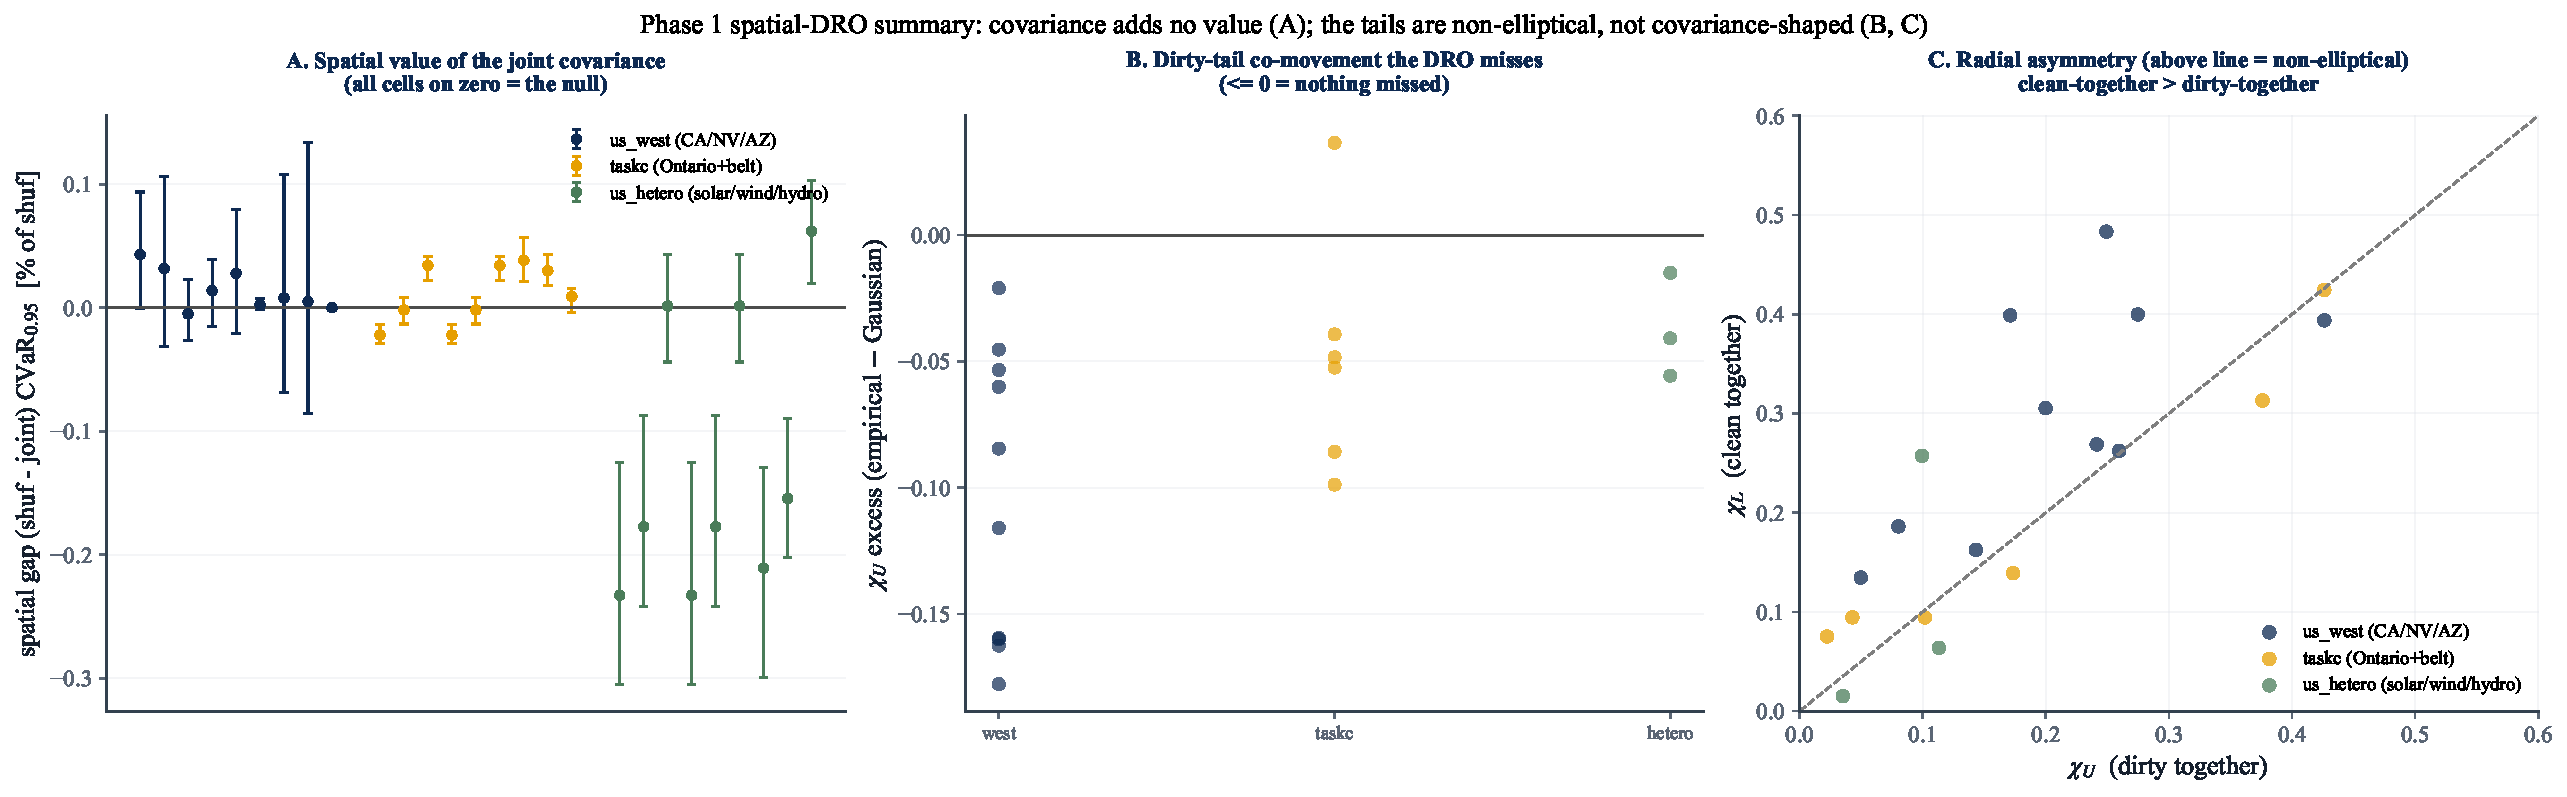
\includegraphics[width=\textwidth]{../figures/case_summary.pdf}
\caption{Phase~1 on one page. \textbf{(A)} spatial gap $\pm$ bootstrap CI for every
case/regime/$\alpha$ cell, clustered on zero --- the null. \textbf{(B)} upper-tail
dependence excess (empirical $-$ Gaussian) $\le 0$ --- no dirty-tail structure is
missed. \textbf{(C)} $\chiL$ vs.\ $\chiU$: points above the diagonal (clean-together
$>$ dirty-together) mark the non-elliptical asymmetry. Regenerate with
\texttt{python -m scripts.plot\_case\_summary}.}
\label{fig:summary}
\end{figure}

\section{Practical recommendation}\label{sec:rec}

For carbon-aware data-center scheduling under a covariance-based robust model,
\textbf{a per-region marginal scheduler captures essentially all the value}.
Modelling cross-region carbon dependence adds estimation burden and, in the
heterogeneous case, measurable noise, for no robust benefit. Spatial dependence
modelling should be reserved for (i) decision structures that can \emph{act} on it
(inter-region workload transfer) and (ii) dependence models that can represent its
actual non-elliptical shape --- both Phase~2 directions.

\section{Conclusion and Phase 2 outlook}\label{sec:conclusion}

Phase~1 is a \emph{specification result}: the second moment of spatial carbon
dependence is both \emph{dominated} (by the mean field) and the \emph{wrong object}
(the dependence is non-elliptical --- upper-tail-independent and radially asymmetric).
This is not a dead end but a precise mandate for Phase~2: model the \textbf{copula},
not the covariance. A vine-copula ambiguity set can represent asymmetric tail
dependence ($\chiL \neq \chiU$, Clayton-type clean-together coupling) that the
Mahalanobis--Wasserstein ground metric cannot express; in parallel, an inter-region
\emph{transfer} channel would give the decision a spatial degree of freedom on which
the joint distribution could finally act. Phase~1 has both falsified the simple
spatial-covariance hypothesis and identified, with evidence, exactly where the
remaining value must lie.

\paragraph{Reproducibility.} All results derive from
\texttt{scripts/run\_case\_experiment.py} (region sets \texttt{us\_west}, \texttt{taskc},
\texttt{us\_hetero}; flags \texttt{-{}-residualize}, \texttt{-{}-shrinkage},
\texttt{-{}-ablate-mean}, \texttt{-{}-test-year}, \texttt{-{}-eps-grid}),
\texttt{scripts/calibrate\_capacity.py}, \texttt{scripts/bh\_correction.py}, and the
diagnostic plotters. Summary tables for every number cited here are archived in
\texttt{docs/results\_snapshots/}.

\end{document}
